\section{Results}
Our primary database is used to reconstruct American Sign Language. 
The database is composed of two continuous
runs of the letters of the 
alphabet, signed by the same actor. We test the database
on various sequences that include ``word'' signs (e.g. boy or girl),
which are not included in the database.

\begin{figure*}[ht]
  \centering
  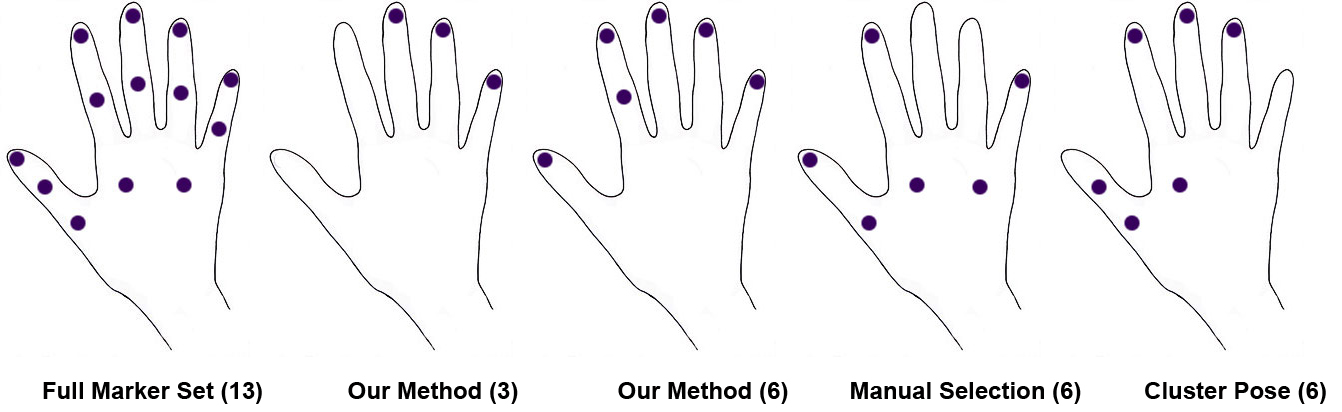
\includegraphics[trim = 0mm 0mm 0mm
0mm,width = \textwidth] {images/marker_sets.jpg} %width=2.5in
  \caption{The tested marker sets.}
  \label{fig:marker_sets}
\end{figure*}


For our sparse marker set, we choose to use six markers as our
baseline in order to compare our technique to existing solutions. 
Using the method described in Section 5 to determine 
marker importance, the markers chosen are all of the fingertips
and one on the lower part of the index finger. When we choose a
marker set of three, the markers chosen are the fingertips of the 
middle, ring, and pinky fingers (Figure ~\ref{marker_sets}).

Our method uses regression to predict principle components for
a sequence of motion. In Figure ~\ref{fig:BabySigns_comps}, we compare
the top three predicted components of a sequence of sign language
to the components of the original sequence with a full marker set. Plots
of the components of six markers and three markers are shown.
Though there are differences, the motion of each component closely
follows that of the ground truth for both marker sets. This can also be seen
in a reconstruced animation in the accompanying video.

We compare our marker set of six to markers sets derived from the manually
selected set, proposed by Hoyet et al. (2011) and the cluster pose error
method proposed by Kang et al.(2012). Using the regression
method, our marker set produces a smaller average joint angle error per frame 
for all of our current sign language tests. Figure
~\ref{fig:3_methods} shows these differences, again using the previous sign 
language clip as an example. The three distinct poses reached
in the sign language clip are also shown using the different marker
sets in Figure ~\ref{fig:BabySigns_methods}. Our marker set is consistently
close to the original pose where as
the two other marker sets fail at achieving at least one pose.

To test the robustness of the database, we attempt to reconstruct 
motions that are not sign language. The motions we test include 
counting and general gesticulations. Our sparse marker set of six
successfully reconstructs counting the numbers 1 through 5, but the marker
set of three fails to reconstruct the number 5. For the gesture based motion,
many of the general poses in the sequence appear to be reached, but the accuracy
of the joint angles is visibly not as good the sign language reconstructions. We
then test to see if the use of another database can improve the gesture
reconstruction. Our method is performed using a gesture database. The selected
sparse marker sets of six and three are different than our previous sets.
Using the gesture database results in high quality gesture reconstructions
for both marker sets of six and three.



\begin{figure}[ht]
  \centering
  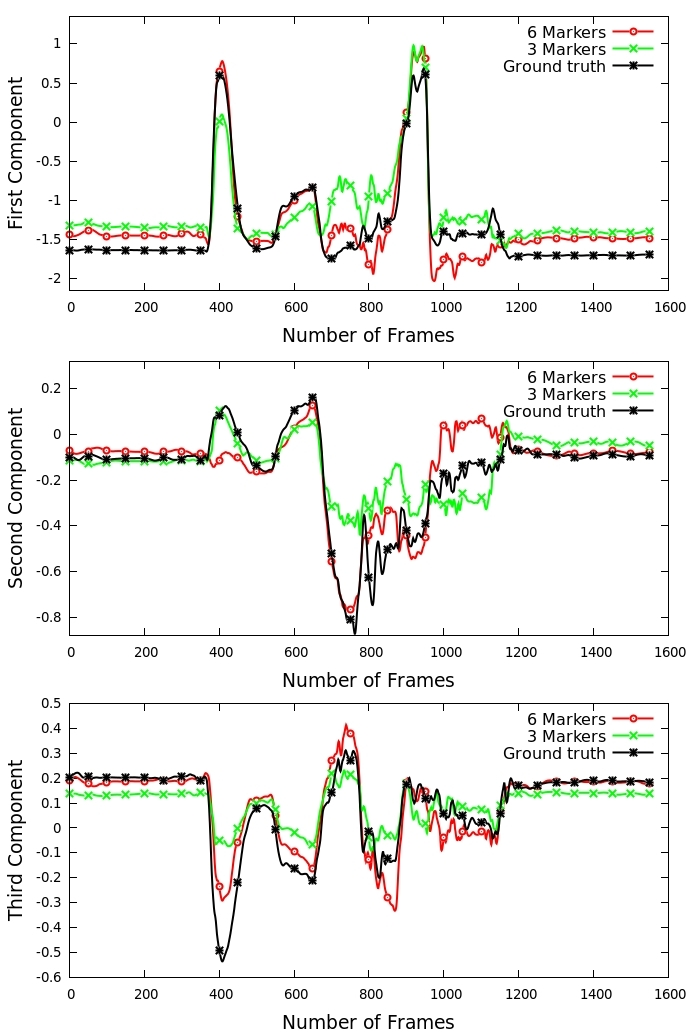
\includegraphics[trim = 28mm 0mm 0mm 0mm,
width=0.45\textwidth]{images/Components_babySigns1.jpg} %width=2.5in
  \caption{Comparison of the components of a reconstructed clip of baby
sign language when using 6 markers and 3 markers. Ground Truth is
the original clip recorded with 13 markers.}
  \label{fig:BabySigns_comps}
\end{figure}

% \begin{figure}[ht]
%   \centering
%   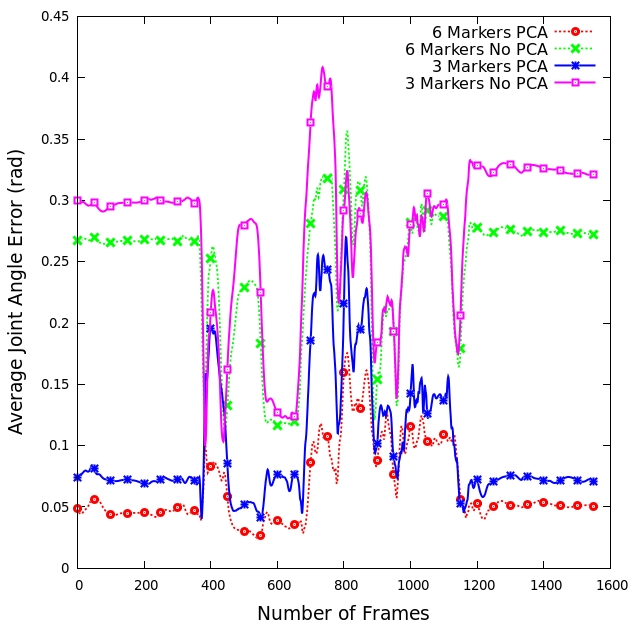
\includegraphics[trim = 28mm 0mm 0mm 0mm,
% width=0.45\textwidth]{images/avgError_6_3_jangles_babySigns1.jpg} %width=2.5in
%   \caption{Comparison of two regression methods: regression to principle
% components and regression to joint angles.}
%   \label{fig:PCA_noPCA}
% \end{figure}

\begin{figure}[ht]
  \centering
  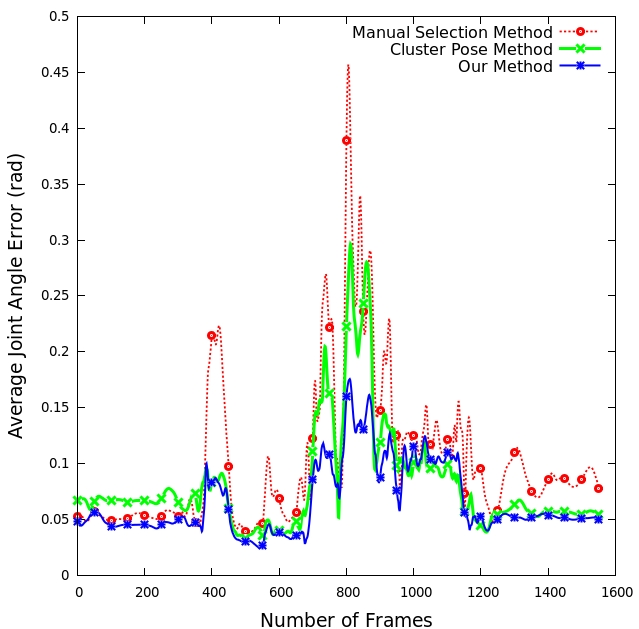
\includegraphics[trim = 28mm 0mm 0mm 0mm,
width=0.45\textwidth]{images/avgError_Marker_sets.jpg} %width=2.5in
  \caption{Comparison of three marker set selection methods that use 6 markers.}
  \label{fig:3_methods}
\end{figure}


\begin{figure}[ht]
  \centering
  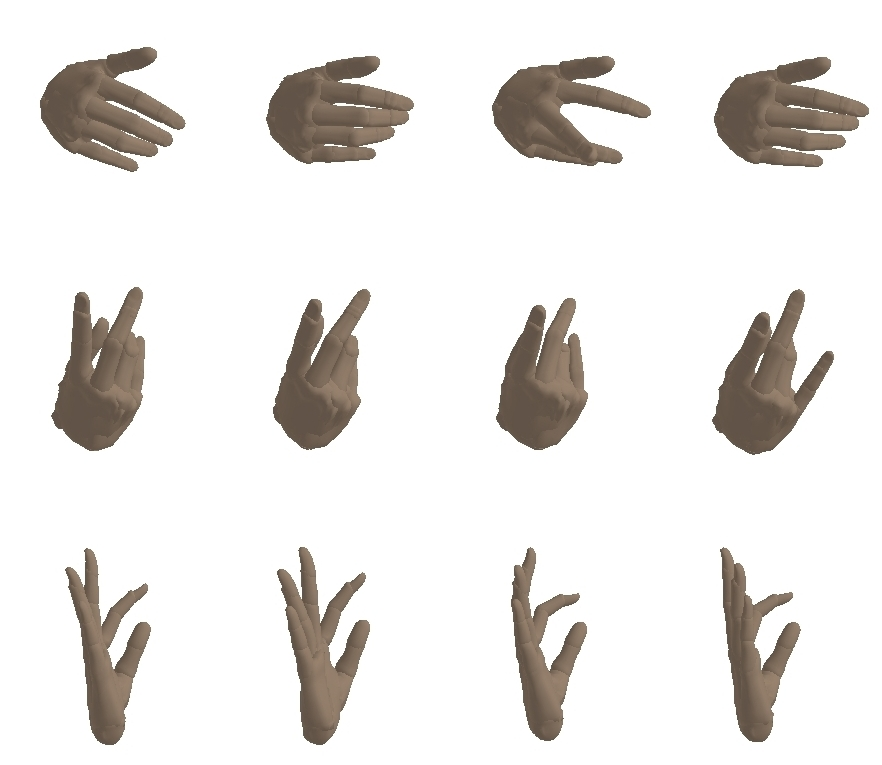
\includegraphics[trim = 28mm 0mm 0mm 0mm,
width=0.45\textwidth]{images/compiled_babySigns1_poses.jpg} %width=2.5in
  \caption{The three distinct poses of the baby sign language clip
reconstructed with the three different marker sets. They are compared to
the original poses.}
  \label{fig:BabySigns_methods}
\end{figure}





